\documentclass{article}
% 设置页面的环境,a4纸张大小,左右上下边距信息
\usepackage[a4paper,left=10mm,right=10mm,top=15mm,bottom=15mm]{geometry}
\usepackage[UTF8]{ctex}
\usepackage{amsmath}
\usepackage{graphicx} % Required for inserting images
\usepackage{subfigure}

\title{Numerical Analysis HW1}
\author{3220103612 章杨}
\date{September 2023}

\begin{document}
\maketitle
\large
\section{Problem1}
引理:Intermediate Value Theorem:

If f$\in$C[a,b] and K is any number between f (a) and f (b), then there exists a number c in (a, b) for which f (c) = K.
\subsection{a.}
不妨假设$f(x_1) \leq f(x_2)$,那么一定有$f(x_1) \leq \frac{f(x_1)+f(x_2)}{2} \leq f(x_2)$,根据介质定理,一定$\exists \xi \in [a,b]$,使得$\frac{f(x_1)+f(x_2)}{2}=f(\xi)$。
\subsection{b.}
不妨假设$f(x_1) \leq f(x_2)$,设$K=\frac{c_1 f(x_1)+c_2 f(x_2)}{c_1+c_2}$,则
    $$\begin{cases}
    f(x_1)-K=\frac{c_2(f(x_1)-f(x_2)}{c_1+c_2}\leq 0\\
    f(x_2)-K=\frac{c_1(f(x_2)-f(x_1)}{c_1+c_2}\geq 0\\
    \end{cases}
    $$
    
得到$f(x_1)\leq K \leq f(x_2)$ ,根据介质定理,一定$\exists \xi \in [a,b]$,使得$f(\xi)=\frac{c_1 f(x_1)+c_2 f(x_2)}{c_1+c_2}$。

\subsection{c.}
取$f(x)=x^2$,令$x_1=1,x_2=2,c_1=2,c_2=-1$,则$\frac{c_1 f(x_1)+c_2 f(x_2)}{c_1+c_2}=-2\notin [f(x_1),f(x_2)]$
\section{Problem2}
\subsection{a.}
absolute error:$|f(x_0)-\Tilde{f(x_0)}|=|f^{'}(\xi) \epsilon|=|f^{'}(x_0+\theta \epsilon) \epsilon|,0<\theta<1$,
当$\epsilon$足够小时,原式=$|f^{'}(x_0) \epsilon|$

relative errors:$|f(x_0)-\Tilde{f(x_0)}|/|f(x_0)|=|f^{'}(\xi) \epsilon|=|f^{'}(x_0+\theta \epsilon) \epsilon|/|f(x_0)|,0<\theta<1$,
当$\epsilon$足够小时,原式=$\epsilon$

\subsection{b.}
$|f(x_0)-\Tilde{f(x_0)}|=|f^{'}(\xi) \epsilon|=|f^{'}(x_0+\theta \epsilon) \epsilon|,0<\theta<1$

i)$f(x)=e^x$

absolute errors:$ (1.359140914229522\times 10^{-5},1.359147709951083 \times 10^{-5})$

relative errors:$(5.000000000000000\times 10^{-6},5.000025000062500\times 10^{-6})$

ii)$f(x)=sin(x)$

absolute errors:$ (2.701490492532310\times 10^{-6},2.701511529340699\times 10^{-6})$

relative errors:$(3.210438079631523\times 10^{-6},3.210463079671654\times 10^{-6})$
\subsection{c.}
i)$f(x)=e^x$

absolute errors:$ (0.110132328974034,0.110132879637055)$

relative errors:$(5.000000000000000\times 10^{-6},5.000025000062499\times 10^{-6})$

ii)$f(x)=sin(x)$

absolute errors:$ (4.195344044802048\times 10^{-6},4.195357645382262\times 10^{-6})$

relative errors:$(7.711730226688204\times 10^{-6},7.711755226784599\times 10^{-6})$

\section{Problem3}
\subsection{a.}
i)exactly:$\frac{17}{15}$

ii)three-digit chopping:1.133=0.113$\times 10^{1}$

relative errors:2.94$\times 10^{-4}$

iii)three-digit rounding:1.133=0.113$\times 10^{1}$

relative errors:2.94$\times 10^{-4}$


\subsection{b.}
i)exactly:$\frac{301}{660}$

ii)three-digit chopping:0.452

relative errors:8.90$\times 10^{-3}$

iii)three-digit rounding:0.453

relative errors:6.71$\times 10^{-3}$




\section{Problem4}
\subsection{a.}
令$f(x)=F(x)-c_1L_1-C_2L_2=O(x^\alpha)+O(x^\beta)$,只需证明$ \lim_{x\to 0} \frac{f(x)}{x^\gamma} =A(A\neq 0)$,
而
$$\lim_{x\to 0} \frac{f(x)}{x^\gamma} =\begin{cases}
    c_1(\alpha\leq\beta)\\
    c_2(\alpha>\beta)\\
    \end{cases}\neq 0$$
    
证毕

\subsection{b.}
令$g(x)=G(x)-L_1-L_2=O(c_1^\alpha x^\alpha)+O(c_2^\beta x^\beta)$,只需证明$ \lim_{x\to 0} \frac{g(x)}{x^\gamma} =A(A\neq 0)$,
而
$$\lim_{x\to 0} \frac{g(x)}{x^\gamma}=\lim_{x\to 0} *(O(x^\alpha)+O(x^\beta))\neq 0$$\\ 

证毕
\section{Problem5}
result:

\begin{figure}[h]
\begin{minipage}[t]{0.3\linewidth}
\centering
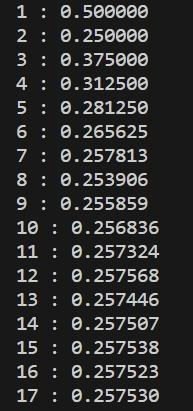
\includegraphics[width=4cm,height=9cm]{5a.png}
\caption{5a}
\end{minipage}
\begin{minipage}[t]{0.3\linewidth}        %图片占用一行宽度的45%
\hspace{2mm}
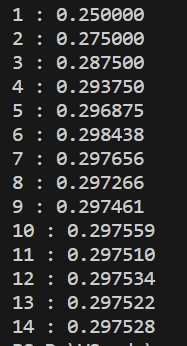
\includegraphics[width=4cm,height=9cm]{5b1.png}
\caption{5b1}
\end{minipage}
\begin{minipage}[t]{0.3\linewidth}        %图片占用一行宽度的45%
\hspace{2mm}
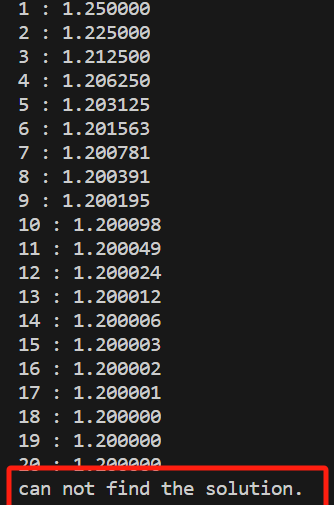
\includegraphics[width=6cm,height=10cm]{5b2.png}
\caption{5b2}
\end{minipage}
\end{figure}

\section{Problem6}
\subsection{a.}
选取g(x)=$(2sin(\pi x)+4 x)/3$,选取原因如下:\\

i)寻找根的大致范围,发现在[1,2]的范围内存在两个根,第一个根的范围在[1,1,3],在寻找g(x)的时候先考虑这一个区间\\

ii)加入参数t,使得$x=\frac{2sin(\pi*x)+tx}{t-1}=g(x)$ 则$g^{'}(x)=\frac{2\pi cos(\pi x)+t}{t-1}$,令$|g^{'}(x)|<1$,可以化简为$-2\leq \frac{2\pi cos(\pi x)+1}{t-1} \leq 0$,取t=4,可以满足要求\\

\begin{figure}[h]
\begin{minipage}[t]{0.45\linewidth}
\centering
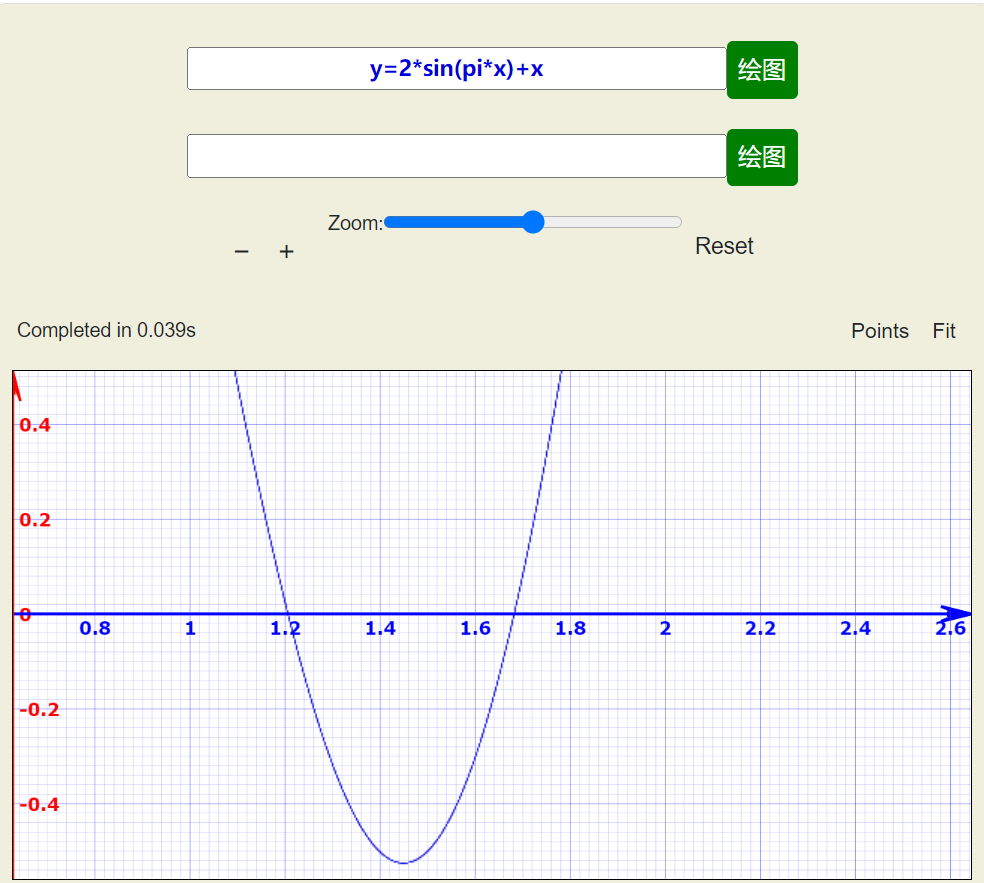
\includegraphics[width=8cm,height=8cm]{6a1.png}
\caption{判断根范围}
\end{minipage}
\begin{minipage}[t]{0.45\linewidth}        
\hspace{2mm}
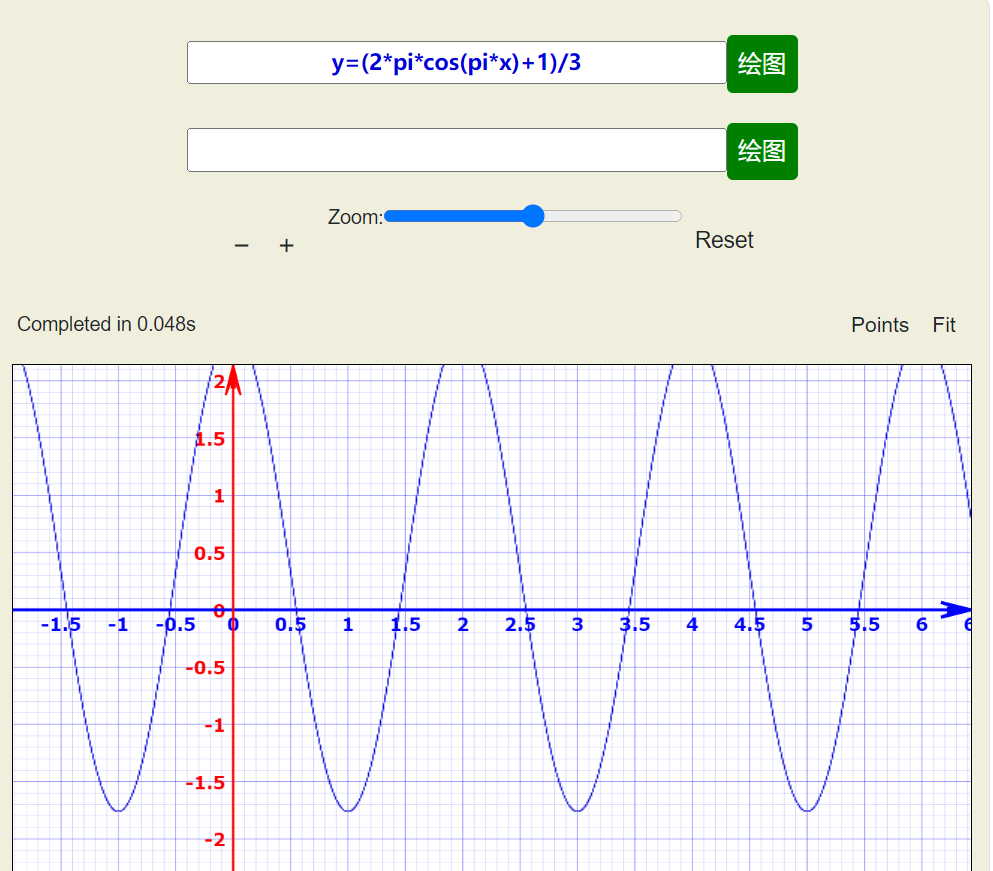
\includegraphics[width=10cm,height=8cm]{6a2.png}
\caption{待定系数t}
\end{minipage}
\end{figure}


结果如图
\begin{figure}[h]
\centering
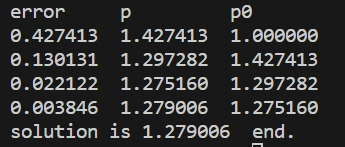
\includegraphics[scale=0.8]{6a3.png}
\caption{6a结果}
\label{figure}
\end{figure}\\

\subsection{b.}
选取$g(x)=\frac{e^{x}}{3x}$,取p0=0.5(这只是一个解,事实上应该有三个解)
\begin{figure}[h]
\centering
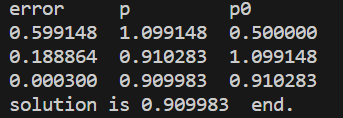
\includegraphics[scale=1.75]{6b1.png}
\caption{6b结果}
\label{figure}
\end{figure}\\



\section{Problem7}
$|p_1-p|\geq |g(p_0)-p|= |g(p_0)-g(p)|=|(p_0-p)g^{'}(p_0+\epsilon(p_0-p)|=|(p_0-p)||g^{'}(p_0+\epsilon(p_0-p)|$,\\

且$|g^{'}(p_0+\epsilon(p_0-p)|>1$,\\

故$|p_1-p|>|(p_0-p)|$

\end{document}

